%\VignetteIndexEntry{Analysis of alternative splicing using ASpli}
%\VignetteKeywords{Alternative splicing analysis}
%\VignettePackage{ASpli}
\documentclass{article}
<<style, echo=FALSE, results=tex>>=
BiocStyle::latex()
options(continue=" ")
@

\usepackage{verbatim} 
\usepackage{caption} 
\usepackage{cite}
\usepackage{subcaption}
\usepackage{hyperref}
\usepackage{amsmath}
\usepackage{float}

\newcommand{\secref}[1]{\ref{#1}:\nameref{#1}}

\newfloat{captionedEq}{thp}{eqc}
\floatname{captionedEq}{Equation}

\title{\texttt{ASpli}: An integrative R package for analysing alternative 
  splicing using RNAseq}

\author{Estefania Mancini, Javier Iserte, Marcelo Yanovsky, Ariel Chernomoretz}

\begin{document}

\SweaveOpts{concordance=TRUE}

\maketitle

\tableofcontents

\section{Introduction}

Alternative splicing (AS) is a common mechanism of post-transcriptional gene 
regulation in eukaryotic organisms that expands the functional and regulatory 
diversity of a single gene by generating multiple mRNA isoforms that encode 
structurally and functionally distinct proteins. The development of novel 
high-throughput sequencing methods for RNA (RNA-Seq) has provided a powerful 
means of studying AS under multiple conditions and in a genome-wide manner 
\cite{pmid24549677}. However, using RNA-seq to study changes in AS under 
different experimental conditions is not trivial. 
In this vignette, we describe how to use ASpli, an integrative and user-friendly
R package that facilitates the analysis of changes in both annotated and novel 
AS events. This package combines statistical information from exon, intron, and 
splice junction differential usage (p-value, FDR), with information from splice 
junction reads to calculate differences in the percentage of exon inclusion 
($\Delta$PSI) and intron retention ($\Delta$PIR). The proposed methodology 
reliably reflect the magnitude of changes in the relative abundance of different 
annotated and novel AS events. This method can be used to analyze both simple 
and complex experimental designs involving multiple experimental conditions.

\section{Getting started}

BAM files of each sample and gene annotation are mandatory. Make sure all files 
use the same coordinate system. It is a good practice to organize all required 
files (or symbolic links of them) together into the  working directory.

\subsection{Installation}
ASpli is available at Bioconductor site and can be downloaded using
\texttt{biocLite()}:
<<installation, echo=TRUE, eval=FALSE>>=
source("https://www.bioconductor.org/biocLite.R")
biocLite("ASpli")
@
%<<loadASpli, echo=TRUE, eval=TRUE>>=
<<loadASpli, echo=TRUE, eval=FALSE>>=
library(ASpli)
@
 
\texttt{biocLite()} will take care of installing all the packages that ASpli 
depends on e.g. edgeR, GenomicFeatures, GenomicRanges, GenomicAlignments, Gviz, 
and other R package required. Some packages depend on operating system
packages, like \texttt{curl}, that are not installed automatically, and should
be installed by the user.

\subsection{Building a \texttt{TxDb} of your genome}
Gene annotation is handled using \texttt{TxDb} objects, which are provided by
\texttt{GenomicFeatures} package. The building of a \texttt{TxDb} object might 
be time consuming, depending on the size of your genome. If a \texttt{TxDb} has
been already created, we strongly recommend saving it as a \texttt{sqlite} file
and reloading it any time the analysis is run. The \texttt{GenomicFeatures} 
package provides functions to create TxDb objects based on data downloaded from
UCSC Genome Bioinformatics, BioMart or gff/gtf files. See "Creating New TxDb 
Objects or Packages" in the \texttt{GenomicFeatures} vignette for more details.
In this example, a TxDb is built from a gtf file:

<<makeTx, echo=TRUE, eval=FALSE>>=
library(GenomicFeatures)
TxDb <- makeTxDbFromGFF(
  file="genes.gtf",
  format="gtf")
@



\section{Running \texttt{ASpli}}

The workflow intended to be used with \texttt{ASpli} is divided in five
steps (Figure \ref{fig:ASpliStructure}). For each of these steps
ASpli provides a single or few functions to use:
\begin{enumerate}
  \item Genomic alignments reading: \texttt{ loadBAM() }
  \item Feature extraction: \texttt{ binGenome() }
  \item Read counting: \texttt{ readCounts() }
  \item Alternative splicing discovery using junctions: \texttt{ AsDiscover() }
  \item DE and DU estimation \texttt{ DUreport(), junctionDUReport() and
  DUreportBinSplice() })
\end{enumerate}

At each step it is possible to export results in a friendly manner. 
See Section \ref{sec:output}:\nameref{sec:output} for more details.

ASpli defines four major objects used to store data and perform operations
ralated to a single task. Throughout this vignette each of these will be
discussed in detail, however they are presented here:
\begin{description}
  \item[ASpliFeatures] Contains data extracted from annotation, such a genomic
  coordindates of genes.
  \item[ASpliCounts] Contains counts of aligned reads to each genomic feature.
  \item[ASpliDU] Contains results of Differential expression and usage analysis.
  \item[ASpliAS] Contains data useful to search novel splicing events.
\end{description}

\begin{figure}[ht!]
\centering
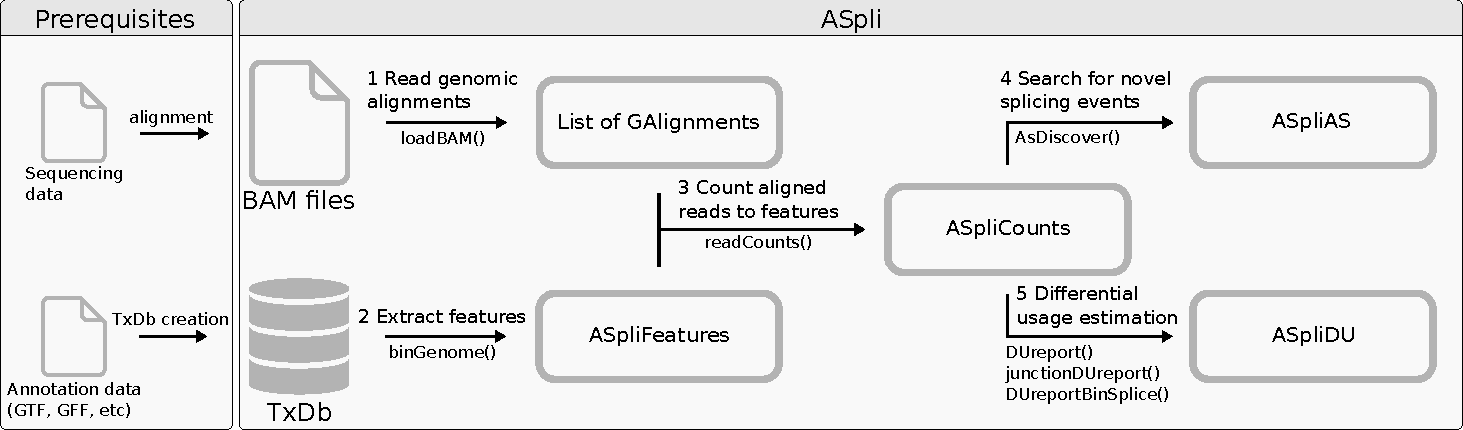
\includegraphics[width=0.8\textwidth]{images/workflow.pdf}
\caption{ Workflow of ASpli pipeline and prerequisites.  Each arrow represents
one of the main steps of a typical analysis. Rounded boxes are objects created
by ASpli functions.  Names under arrows are functions included in ASpli used to
generate each kind of object. }
\label{fig:ASpliStructure}
\end{figure}

\subsection{To BIN or not to BIN }
% Agregar definicion de los bins Io
\label{sec:binDefinition}
Sub-genic features such as exons and introns are analyzed using existing
annotations by splitting the genome into non-overlapping features called bins, 
as described previously for DEXSeq \cite{pmid22722343}. Exon and intron 
coordinates are then extracted from the annotation, but only those from 
multi-exonic genes are saved for further evaluation. When more than one isoform 
exists, some exons and introns will overlap. Exons and introns are then 
subdivided into new features called exon and intron bins, and are then 
classified into exclusively exonic bins, exclusively intronic bins, or 
alternative splicing (AS) bins (See Figure \ref{fig:binDefinition}). 
In addition to these non overlapping bins, an additional type of bin is also
defined. The latter corresponds to full introns extracted from annotation,
before they are splitted by the presence of overlapping exons in another
isoform. These bins as referred as \texttt{Intron original} bins.

\begin{figure}[ht!]
\centering
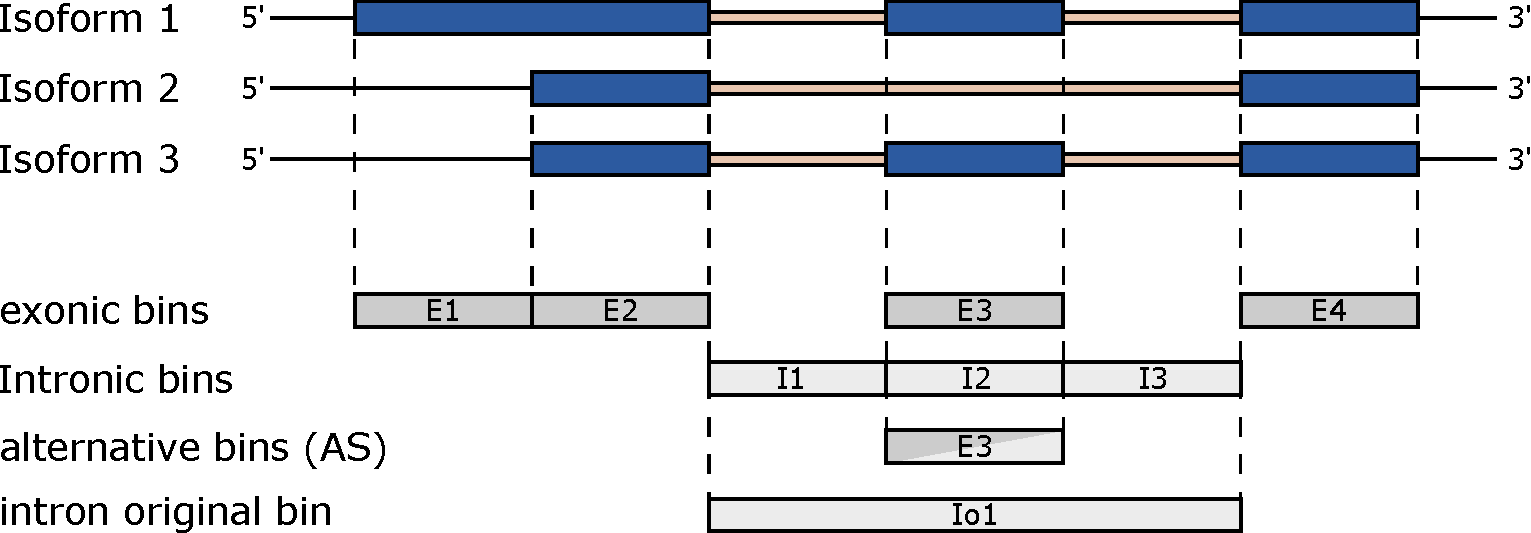
\includegraphics[width=12cm]{images/binDefinition.pdf}
\caption{ Schema of resulting bins from a gene with three hypothetical
  transcripts. Those bins that are exonic and intronic in different isoforms are 
  named \textit{AS bins}.
}
\label{fig:binDefinition}
\end{figure}

Annotated junctions from all the transcripts are also reported. Junction 
coordinates are defined as the last position of the five prime exon (donor 
position) and first position of the three prime exon (acceptor).

\subsubsection{Splicing event assignation} \label{sec:eventAssign}
Each AS bin is then assigned to a kind of splicing event. The assignation is
made using the minimum gene model corresponding to the bin being evaluated and
the two neighbor bins (one to the left, one to the right). The minimum gene
model is constructed by extracting from the corresponding isoforms the
regions of the selected bins and removing those that are identical. The criteria
for the assignation is that the assigned splicing event should explain in the
most simple way a potential differential usage found for this bin alone. When
the minium gene model contains two isoforms the bin is labelled as follow:

\begin{itemize}
  \item \textbf {ES} Exon skipping
  \item \textbf {IR} Intron retention
  \item \textbf {ALt5'SS} Alternative 5' splicing site
  \item \textbf {ALt3'SS} Alternative 3' splicing site
\end{itemize}

When the minimum gene model contains three, four or five isoforms (note that no
more than five non redundant isoforms can exist in the minimum gene model)
labels of bins is similar to previous but have an '*' character added to end
( \textbf{ES*}, \textbf{IR*}, \textbf{Alt5'SS*}, \textbf{Alt3'SS*}) in order to
show that multiple isoforms exists and, therefore, the results should be used
with caution. In some cases, this is not possible to make an assignation for a
bin with assumptions made here, those bins are labelled as \textbf{as}. The
figure \ref{fig:binAssignation} shows a summary of the assignation.
Finally, those bins that are at the beggining or end of a transcript are
labelled as \textbf{external}.

\begin{figure}[ht!]
\centering
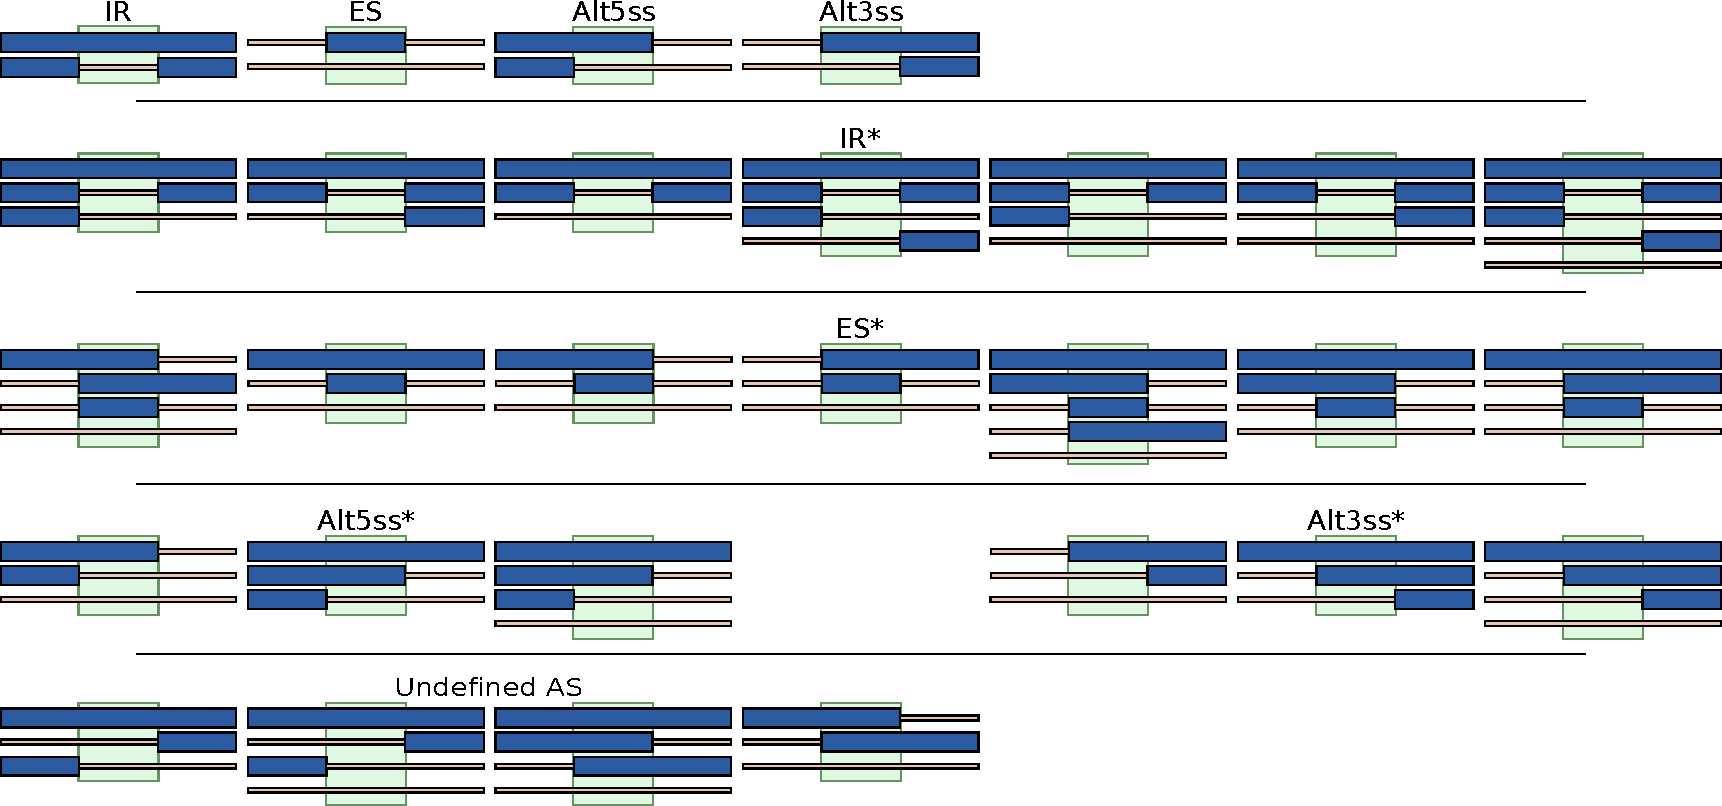
\includegraphics[width=0.9\textwidth]{images/event_assignment.pdf}
\caption{ Summary of assignation of splicing events to bins from minimum gene
model. The bin being evaluated has a green background highlight. The blue boxes
represents exons, while the little light orange boxes represent introns. Gene
models shown are plus sense strand. }
\label{fig:binAssignation}
\end{figure}



\subsubsection{Naming conventions for bins and junctions }
\label{sec:binNaming}
Subgenic features are named as follow for a hypothetical gene named GeneAAA:
\begin{itemize}
  \item \textbf{GeneAAA:E001}: defines first exonic bin
  \item \textbf{GeneAAA:I001}: defines first intronic bin
  \item \textbf{GeneAAA:Io001}: defines first \texttt{Intron original} before 
  being divided
  \item \textbf{GeneAAA:J001}: defines first junction
\end{itemize}

Bins and junctions are consecutively named from 5' to 3' sense of the plus
strand of the reference sequence. This implies that  bins and junctions with
lower numbering are always closer to the 5' of that strand. Alternative splicing
bins are named as exons.

All tasks presented in this section, subgenic splitting of genes into
bins, coordinates extraction of junctions, genes and bins, naming of genes and
bins and splicing event assignation to bins are performed by single method
: \texttt{binGenome}. The result is an object of class \texttt{ASpliFeatures}.
\texttt{binGenome} methods accepts and additional optional argument
\texttt{geneSymbols} used to assign symbols (i.e. common name or a short
description) to genes.
Then, features cordinates could be obtained using their accesors methods.
Method \texttt{ featuresg } returns coordinates for genes as a GRangesList
object, and methods \texttt{ featuresb } and \texttt{ featuresj } returns
coordinates for bins and bins respectively as a GRanges object. GRangesList an
GRanges are objects defined in GenomicRanges package. These objects contains
aditional information stored as metadata and can be accessed with \texttt{mcols}
function.

<<binGenome, echo=TRUE, eval=FALSE>>=
# extract features from annotation
features      <- binGenome( aTxDb ) 

# Accesors of ASpliFeatures object 
geneCoord     <- featuresg( features )
binCoord      <- featuresb( features )
junctionCoord <- featuresj( features )
# Extract metadata annotation, such as bins names, event and feature type, 
# locus name.  
binMetadata   <- mcols( binCoord )
@

<<binGenome, echo=TRUE, eval=FALSE>>=
# extract features and map symbols to genes
symbols       <- data.frame( row.names = genes( aTxDb ), 
                             symbol = paste( 'This is symbol of gene:',
                                             genes( aTxDb ) ) )
features      <- binGenome( aTxDb, geneSymbols = symbols ) 
@

\subsection{Defining the targets }
\label{sec:targetsDef}

Before to proceed with counting of aligned reads by feature, is required
to define the samples, the experimental factors and to associate them with the
corresponding genomic alignment files. This must be specified in a 
\texttt{data.frame} that has as many rows as samples. Each row name is the name
of a sample. The first column must be named \texttt{bam} and contain the path to
a single bam file. The remaining columns are used to define the experimental
factors for each sample and must have a proper name. This \texttt{data.frame} is
referred to as the \textbf{targets} \texttt{data.frame}. 

For example, for a one factor experiment with 2 replicates for each condition 
(Control and Mutant) the  \textbf{targets} \texttt{data.frame} can be defined as 
follow:
%<<targetsDF, echo=TRUE, eval=TRUE>>=
<<targetsDF, echo=TRUE, eval=FALSE>>=
bamFiles <- c( "Ct1.bam", "Ct2.bam", "Mut1.bam","Mut2.bam" )
targets <- data.frame( row.names =  c("CT_rep1","CT_rep2", "Mut_rep1", "Mut_rep2"),
                       bam = bamFiles,
                       genotype = c("CT","CT", "Mut", "Mut") , 
                       stringsAsFactors = FALSE )
@ 

More sofisticated designs should be specified as follow. For example: for a two
factor experiment with 2 replicates for each condition (Control, Mutant, Time1,
Time2).

%<<targetsDF2, echo=TRUE, eval=TRUE>>=
<<targetsDF2, echo=TRUE, eval=FALSE>>=
bamFiles <- c("Ct_time1_rep1.bam", "Ct_time1_rep2.bam",
              "Ct_time2_rep1.bam", "Ct_time2_rep2.bam",
              "Mut_time1_rep1.bam","Mut_time1_rep2.bam",
              "Mut_time2_rep1.bam","Mut_time2_rep2.bam")

targets_2 <- data.frame( row.names = c( 'CT_t1_r1',  'CT_t1_r2',
                                        'CT_t2_r1',  'CT_t2_r2',
                                        'Mut_t1_r1', 'Mut_t1_r2',
                                        'Mut_t2_r1', 'Mut_t2_r2' ),
                         bam = bamFiles,
                         genotype = c( 'CT',  'CT',  'CT',  'CT', 
                                       'MUT', 'MUT', 'MUT', 'MUT' ),
                         time     = c( 't1', 't1', 't2', 't2', 
                                       't1', 't1', 't2', 't2' ),
                         stringsAsFactors = FALSE )
@

The name of the each experimental condition is determined by the experimental
factors defined in the \textbf{targets} \texttt{data.frame}. Those can be
consulted using the \texttt{getConditions} function. 

<<targetsDF2, echo=TRUE, eval=FALSE>>=
# Show the name of each unique condition in the console
getConditions( targets_2 )
@

\subsection{Read Counting }

\subsubsection{Mapping file and bam loading } 

Once the \textbf{targets} \texttt{data.frame} is defined the alignment data
from bam files can be loaded easily with \texttt{loadBAM} function. BAM files
are loaded and stored as a named list of \texttt{GAlignments} objects.
\texttt{GAlignments} objects are defined in \texttt{GenomicAlignments} package.

<<loadBam, echo=TRUE, eval=FALSE>>=
bam <- loadBAM(targets)
@

\subsubsection{Counting alignment reads overlapping features } 

Using the method \texttt{readCounts}, read alignments are overlaid on features.
Results are stored into an \texttt{ASpliCounts} object. Read densities are
calculated for genes and bins as shown below:
\begin{equation*}{
  f_{d} = \frac{ N_{r} }{ l }
}
\end{equation*}

Where $f_{d}$ is the deature read density, $N_{r}$ is the number of reads
overlaping the feature and $l$ is the length of the feature.

Tables containing counts and read densities are produced at different
genomic levels, including genes, bins, junctions, and intron flanking regions.

The usage of this method is shown below:

<<readCounts, echo=TRUE, eval=FALSE>>=
counts <- readCounts ( 
    features, 
    bam, 
    targets, 
    cores = 1, 
    readLength = 100L, 
    maxISize = 50000,
    minAnchor = NULL )
@
Where the accepted parameters are:

\begin{itemize}
  \item \texttt{features}: An ASpliFeatures object. 
  \item \texttt{bam}: A list of \texttt{GAlignments} generated with loadBAM
\texttt{function}.
  \item \texttt{targets}: A \textbf{targets} \texttt{data.frame} as defined in
section \nameref{sec:targetsDef}. 
  \item \texttt{cores}: Number of proccessor cores used to speed up the
computation.
  \item \texttt{readLength}: Read length of sequenced library 
  \item \texttt{maxISize}: maximum intron expected size. Junctions longer than
this size will be dicarded \cite{Hong01122006}.
  \item \texttt{minAnchor}: minimum anchoring overlap for intron flanking
  regions (see \nameref{sec:intronFlanking} ). 
\end{itemize}

The result of \texttt{readCounts} method is an object of class 
\texttt{ASpliCounts}. Count and read density data could be extracted from it as
\texttt{data.frame} objects using accesors methods. Also, it is possible to 
export count and read densities tables to text files in a tidy manner.

<<readCountAccessors, echo=TRUE, eval=FALSE>>=
# Accessing count and read density data
GeneCounts <- countsg(counts)
GeneRd <- rdsg(counts)

BinCounts <- countsb(counts)
BinRd <- rdsb(counts)

JunctionCounts <- countsj(counts)
e1iCounts <- countse1i(counts)
ie2Counts <- countsie2(counts)

# Export count data to text files 
writeCounts(counts=counts, output.dir = "example")
writeRds(counts=counts, output.dir = "example")
@


\subsubsection{Counting intron flanking regions }
\label{sec:intronFlanking}

Every intron is considered as a potential retained intron. Analysis of putative
IR events consider adjacent 5' and 3' exons (E1 and E2, respectively) and the
intron itself (I). Following \cite{ pmid25258385 }, two retention regions E1I 
(connecting exon E1 and I) and IE2 (connecting the intron and exon 2) and one
constitutive (i.e., no retention) junction, E1E2 (connecting exons 1 and 2) are
defined. The read length of sequenced library is used for the definition of 
those new artifitial ranges:

\begin{itemize}
  \item E1I: intron start - (readLength - minAnchor) - intron start + (
  readLength - minAnchor )
  \item IE2: intron end - (readLength - minAnchor) - intron end + ( readLength -
  minAnchor )
  \item \texttt{ minAnchor } is 10\% of read length by default (parameter
  \texttt{minAnchor} )
\end{itemize}

Only those reads which minimum overlap \textit{readLength} and without gap in 
this interval are considered. Accordingly, only sequences aligned within those 
two exons/introns are counted.

\subsubsection{Additional details of \texttt{readCounts} method }

Number of reads by gene are computed summarizing the reads of the constitutive 
exon bins of each gene.
%Nota: no estoy seguro a que llama aca exones constitutivos.

In order to estimate read densities, an effective length (sum of the length of 
exonic bins (constitutive and alternative of their corresponding gene) is
considered.

The minimum overlap length between read and feature is 1. Hence, some reads
might overlap to more than one bin  and could be counted several times.

Junctions are extracted from BAM files. They are defined as those reads
aligned skipping region from the reference (N operator of CIGAR notation
for aligned reads \cite{pmid19505943} ). They are essential for alternative
splicing event quantification and discovery. Junction alignment
quality/confidence is extremely important and it should be controlled at the
moment of the alignment step.

\subsubsection{Contents of ASpliCounts object }
\label{sec:countsContents}
Accessor methods of \texttt{ ASpliCounts } object return \texttt{data.frame}
objects for genes counts, genes read density, bin counts, bin read density, E1I
flanking region counts and IE2 flanking region counts. All of them share the
same structure, however the specific content is different for each kind of 
feature. The first columns contains feature information extracted from the
annotation, and then there several columns with count and read density data for
each experimental sample. A more detailed overview is shown below:

\begin{itemize}
  \item Gene counts and gene read densities \texttt{data.frames} contains the
  following columns:
    \begin{description}
      \item[row.names] Gene name as is found in annotation.
      \item[symbol] An optional common name for the gene, that must be provided at
      the moment of feature extraction (see section \ref{sec:binDefinition}:\nameref{sec:binDefinition}).
      \item[locus\_overlap] Show the names of all other overlapping \textit{loci}.
      \item[gene\_coordinates] Show the genomic coordinates of the gene with
      format \texttt{chromosome:start-end}.
      \item[start] Left-most position of the gene.
      \item[end] Right-most position of the gene.
      \item[length] Number of bases covering the gene.
      \item[effective\_length] Number of bases that overlaps with annotated exons.
      \item[sample data] One column by sample containing gene counts or gene read
      densities.
      \\
    \end{description} 
  \item Bin counts and bin read densities \texttt{data.frames} contains the
  following columns:
    \begin{description}
      \item[row.names] Bin name as given in section \ref{sec:binNaming}:\nameref{sec:binNaming}.
      \item[feature] Is the kind of bin: \textbf{E} for exonic bins, \textbf{I}
      for intronic bins and \textbf{Io} for introns before splitting.
      \item[event] Splicing event asigned to the bin (see section
      \ref{sec:binDefinition}:\nameref{sec:eventAssign})
      \item[locus] The name of the locus that contains the bin.
      \item[locus\_overlap] Show the names of all other overlapping \textit{loci}.
      \item[symbol] An optional common name for the gene, that must be provided at
      the moment of feature extraction (see section \ref{sec:binDefinition}:\nameref{sec:binDefinition}).
      \item[gene\_coordinates] Show the genomic coordinates of the gene with
      format \texttt{chromosome:start-end}.
      \item[start] Left-most position of the bin.
      \item[end] Right-most position of the bin.
      \item[length] Number of bases covering the bin.
      \item[sample data] One column by sample containing bin counts or bin read
      densities.
      \\
    \end{description}
  \item Junction count \texttt{data.frame} contains the following columns:
    \begin{description}
      \item[row.names] Junction name in format \texttt{chromosome.5'site-3'site}.
      \item[junction] If junction coincides with a junction inferred
      from the annotation, the name is shown as is given in section
      \ref{sec:binNaming}:\nameref{sec:binNaming}, otherwise contains \texttt{noHit}.
      \item[gene] The name of the locus that contains the junction.
      \item[strand] Sense strand of the gene.
      \item[multipleHit] Contains \texttt{yes} if junction spans multiple genes.
      \item[symbol] An optional common name for the gene, that must be provided at
      the moment of feature extraction (see section \ref{sec:binDefinition}:\nameref{sec:binDefinition}).
      \item[gene\_coordinates] Show the genomic coordinates of the gene with
      format \texttt{chromosome:start-end}.
      \item[bin\_spanned] The names of the bins spanned by the junction.
      \item[j\_within\_bin] If junction fall within a single bin, the name of
      that bin is shown.
      \item[sample data] One column by sample containing junction counts.
      \\
    \end{description}
  \item E1I and IE2 flanking region count \texttt{data.frame} contains the
  following columns:
    \begin{description}
      \item[row.names] Junction name in format \texttt{chromosome.5'site-3'site}.
      \item[junction] If junction coincides with a junction inferred
      from the annotation, the name is shown as is given in section
      \ref{sec:binDefinition}:\nameref{sec:binDefinition}, otherwise
      contains \texttt{noHit}.
      \item[gene] The name of the locus that contains the junction.
      \item[strand] Sense strand of the gene.
      \item[multipleHit] Contains \texttt{yes} if junction spans multiple
      genes.
      \item[symbol] An optional common name for the gene, that must be provided at
      the moment of feature extraction (see section \ref{sec:binDefinition}:\nameref{sec:binDefinition}).
      \item[gene\_coordinates] Show the genomic coordinates of the gene with
      format \texttt{chromosome:start-end}.
      \item[bin\_spanned] The names of the bins spanned by the junction.
      \item[j\_within\_bin] If junction fall within a single bin, the name of
      that bin is shown.
      \item[sample data] One column by sample containing junction counts.
      \\
    \end{description}
    
\end{itemize}

\subsection{Alternative splicing analysis and discovery using junction }

Count data of bins and junctions, generated with \texttt{readCounts} method, can
be used to get an integrative view of the alternative splicing events. The 
method \texttt{AsDiscover} will produce an \texttt{ASpliAS} object containing
comprehensive results of evidence of alternative splicing usage of bins and
junctions. 

The analysis will consider junctions that are completely included within a
unique gene and have more than a minimum number of reads supporting them, by
default this number is five.

For each experimental junction identified, it is also reported if it is novel
and which bins are spanned. In addition, it is stated if the junction is completely
included in an annotated bin, which would indicate that the AS event is a
possible exintron \cite{pmid25934563}.

<<AsDiscover, echo=TRUE, eval=FALSE>>=
as <- AsDiscover( counts, targets, features, bam, readLength=100L, threshold =
5)
@
Where the accepted parameters are:
\begin{itemize}
  \item \texttt{counts}: An ASpliCount object.
  \item \texttt{targets}: A \textbf{targets} \texttt{data.frame} as defined in
section \nameref{sec:targetsDef}.  
  \item \texttt{features}: An ASpliFeatures object. 
  \item \texttt{bam}: A list of \texttt{GAlignments} generated with loadBAM
\texttt{function}.
  \item \texttt{readLength}: Read length of sequenced library 
  \item \texttt{threshold}: minimum number of reads supporting a junction.
  \item \texttt{cores}: Number of proccessor cores used to speed up the
computation.
\end{itemize}

The contents of an \texttt{ASpliAS} object can be retrieved using accessor
methods: \texttt{irPIR}, \texttt{altPSI}, \texttt{esPSI},
\texttt{joint} \texttt{junctionPIR}, \texttt{junctionPSI} (see section
\secref{secASpliAsContent} for a detailed description of each method and retrieved data). In addition, method
\texttt{writeAS}, allows to easily export all the data into text files tables.


<<writeAS, echo=TRUE, eval=FALSE>>=
# Access result from an ASpliAS object 
irPIR  <- irPIR( as )
altPSI <- altPSI( as )
esPSI  <- esPSI( as )
junctionsPIR <- junctionsPIR( as )
junctionsPSI <- junctionsPSI( as )
allBins      <- joint( as )

# Export results to files
writeAS(as=as, output.dir="example")
@

\subsubsection{PIR and PSI metrics}
\label{sec:psir}
To provide an integrative view of the AS events being analyzed, splice junction
information is used to analyze differential bin usage. PSI (percent of
inclusion) and PIR (percent of intron retention) metrics, which are extensively
used to quantify AS \cite{pmid21057496}, are calculated (see figure
\ref{fig:pirEq} ) for bins junctions. Only junctions that pass an abundance
filter are considered for PSI/PIR calculation. The minimum value of
counts for a given junctions and condition is calculated:

\begin{equation}
  J^{min}_{ij} = min( J_{ij} )
\end{equation}
Where $J^{min}_{ij}$ is the minimum value count for junction $i$ in condition
$j$, and $J_{ij}$ is the set of junction supporting reads count values for
junction $i$ in condition $j$. Then, a junction $i$ is kept if $J^{min}_{ij}$ is 
greater or equal than a threshold value for at least one condition $j$.


\begin{figure}[ht!]
    \begin{subfigure}[t]{1\textwidth}
    \centering
      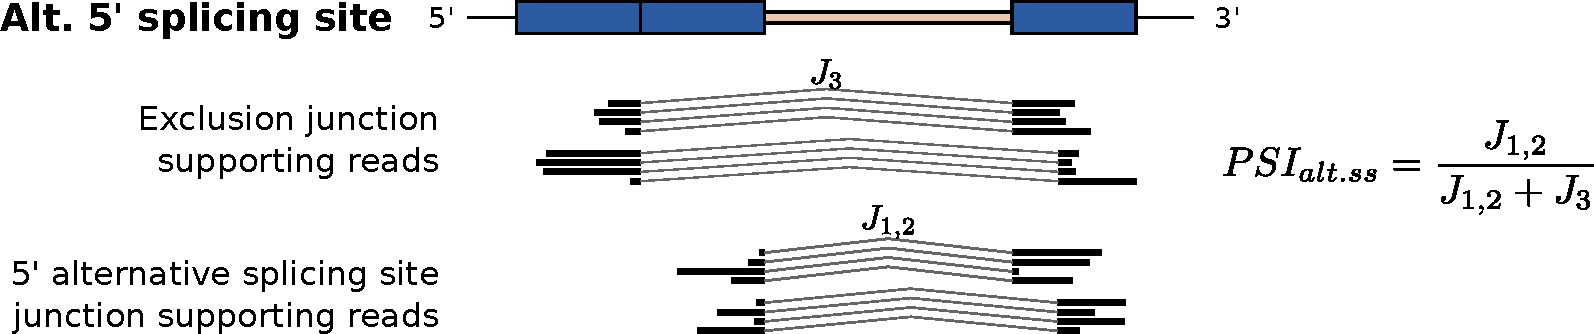
\includegraphics[width=0.7\textwidth]{images/psi5ss.pdf}
      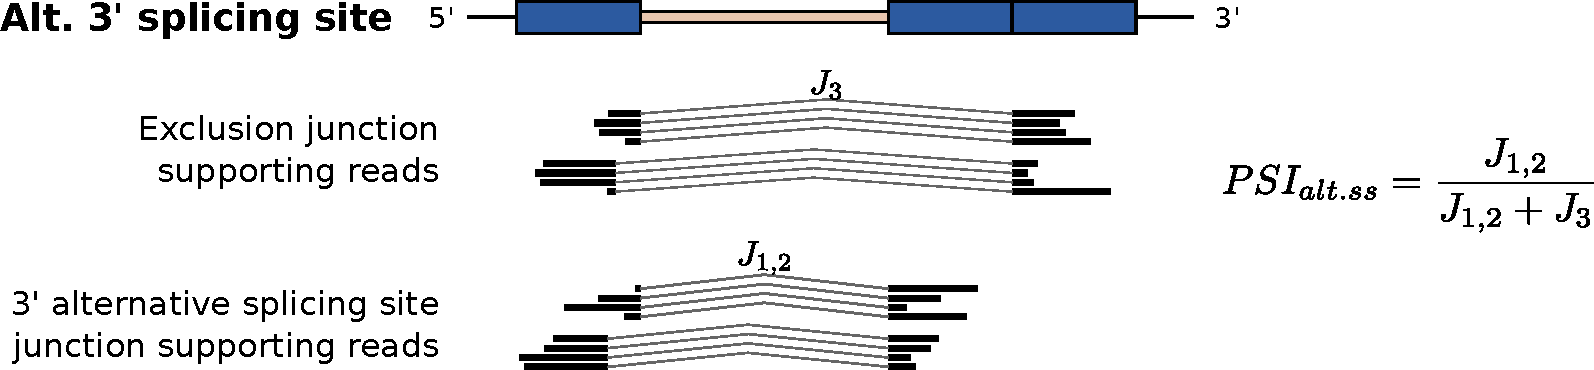
\includegraphics[width=0.7\textwidth]{images/psi3ss.pdf}      
      \caption{PSI metric for alternative 5' and 3' splicing sites estimation and its relationship with junctions}
    \end{subfigure}
    \begin{subfigure}[t]{1\textwidth}
    \centering
      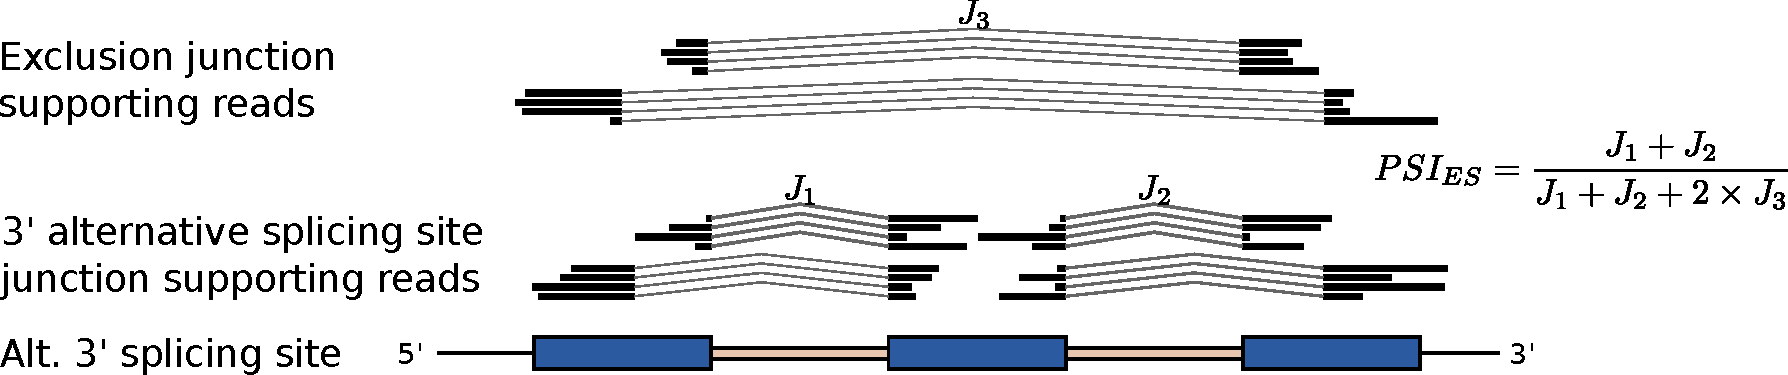
\includegraphics[width=0.7\textwidth]{images/psies.pdf}
      \caption{PSI metric for exon skipping estimation and its relationship with
      junctions}
    \end{subfigure}
    \begin{subfigure}[t]{1\textwidth}
      \centering
      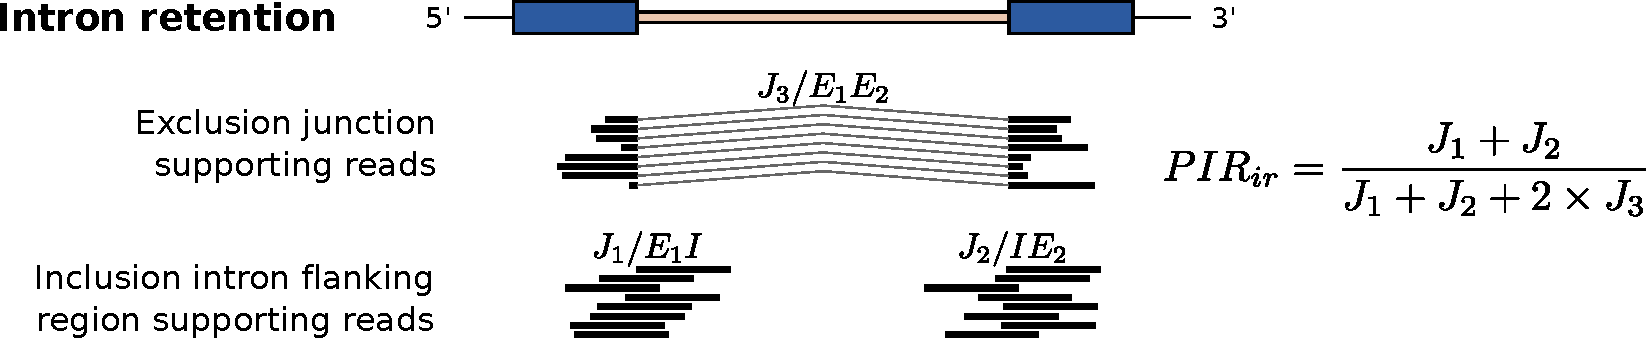
\includegraphics[width=0.7\textwidth]{images/pir.pdf}
      \caption{PIR metric for intron retention estimation and its relationship
      with junctions}
    \end{subfigure}    
    \caption{PSI and PIR metrics estimation and their relationship with
    junctions}
    \label{fig:pirEq}
\end{figure}

For each bin, one of PIR or PSI variants metrics is calculated, the decision of
which one is selected depends on the splice event assigned to that bin (see
section \secref{sec:eventAssign}). If no splice event is assigned, meaning that
the bin is not alternative, an exon are considered to be involved in
a putative exon skiping splicing event, and an intron are considered to be
involved in a putative intron retention splicing event. 

Every junction implies the existence of an intron that could be potentially 
retained, therefore a PIR value is computed for every junction. Also, every
junction defines a 5' and a 3' splicing site. Each one of these can be found
exclusively in this junction or found also in other junctions. The latter is
evidence of an exon skipping event or and alternative 5' or 3' splicing site
event. Althought is not possible to infer the kind of event, the computation of
a PSI value is helpful to detect this cases. The details of the formulas used to
calculted these values are shown in \ref{fig:psir_junc}

This information allows the user to obtain reliable information on the relative
abundance of the AS event being evaluated. Both metrics strongly enrich the 
count-centric analysis and provide independent experimental support for the 
existence of novel AS events, based on the identification of corresponding 
changes in nearby splice junctions.

\begin{figure}
  \begin{subfigure}[t]{1\textwidth}
    \centering
    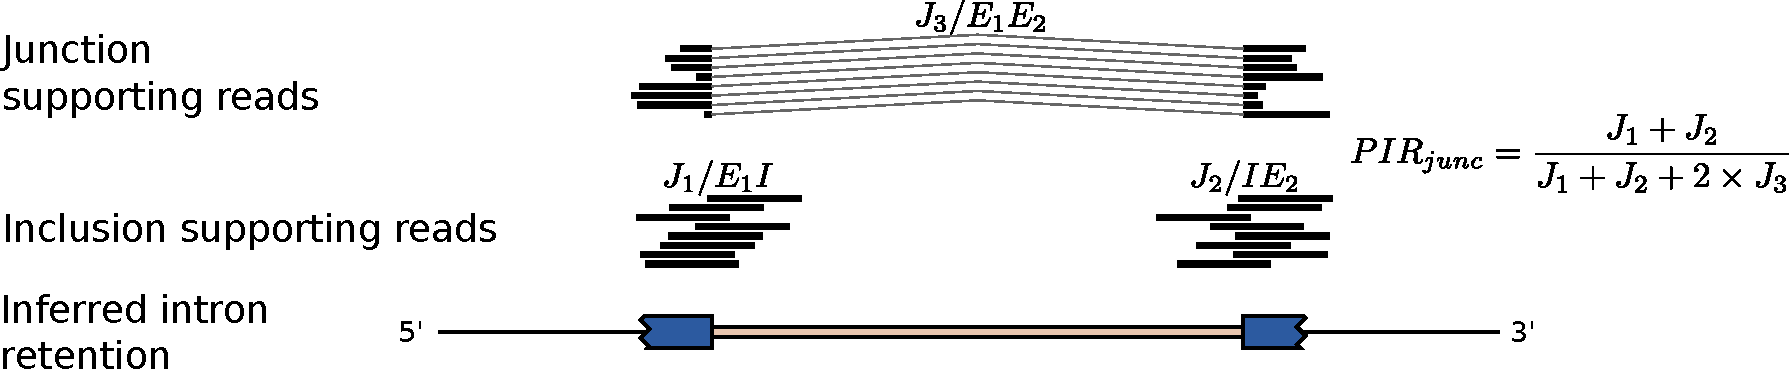
\includegraphics[width=0.7\textwidth]{images/pir_junc.pdf}
    \caption{ PIR metric to estimate intron retention for junctions}
  \end{subfigure}
  \begin{subfigure}[t]{1\textwidth}
    \centering
    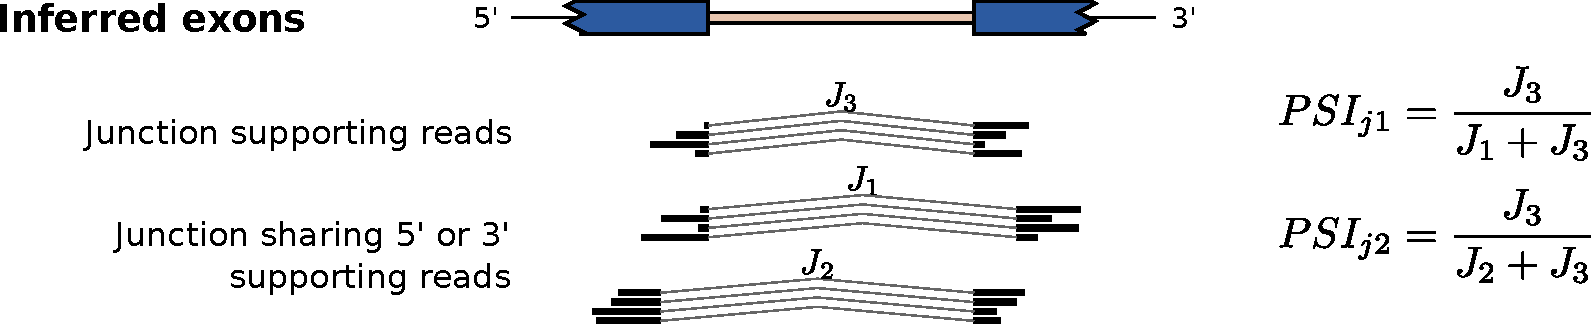
\includegraphics[width=0.7\textwidth]{images/psi_junc.pdf}
    \caption{ PSI metric to compute inclusion of exons bearing a junction.} 
  \end{subfigure}
  \caption{PSI and PIR metrics for junctions}
  \label{fig:psir_junc}
\end{figure}


\subsubsection{New splicing events discovery} 
\texttt{ASpli} allows novel AS events to be identified based on the splice
junction repertoire. A novel AS event can be is identified whenever a
novel splice junction that shares its beginning or end with another splice 
junction is discovered. When a novel AS event is identified using the splice
junction repertoire, the PSI metric is calculated and reported. This ability to
detect novel AS events and to estimate the magnitude of the changes in the usage
of these AS events under different experimental conditions are original
functions of the package.

\subsubsection{Contents of ASpliAS object}
\label{secASpliAsContent}

Accessor methods of \texttt{ ASpliAS } object return \texttt{data.frame}
objects containing detailed information for bins involved in intron retention,
5' or 3' alternative splicing site and exon skipping events, and for
experimental junctions. 

\begin{itemize}
  \item Results for bins involved in intron retention, alternative 5' or 3'
  splicing site, and exon skipping events can be accessed with \texttt{irPIR},
  \texttt{altPSI} and \texttt{esPSI} respectively, or using \texttt{joint}
  method for all of them altogether. These methods return a \texttt{data.frame}
  object which columns are specified below. The description given uses
  \textbf{J1}, \textbf{J2}, \textbf{J3} count values, which have different
  meaning for different metrics, see figures \ref{fig:pirEq} and
  \ref{fig:psir_junc} for more detail.
    \begin{description}
      \item[row.names] Bin name as is defined in \secref{sec:binNaming}.
      \item[event] Splicing event asigned to the bin (see section
      \ref{sec:binDefinition}:\nameref{sec:eventAssign})
      \item[J1] The name of J1 junction or E/I flanking region.
      \item[sample data for J1] J1 counts for each sample.
      \item[J2] The name of J2 junction or E/I flanking region.
      \item[sample data for J2] J2 counts for each sample.
      \item[J3] The name of J3 junction or E/I flanking region.
      \item[sample data for J3] J3 counts for each sample.
      \item[PSI or PIR data] A column by condition with the corresponding PSI
      variant metric or PIR metric.
      \\
    \end{description}
  \item Results for experimental junctions assuming that they correspond to
  introns involved in intron retention events can be accessed with
  \texttt{junctionPIR} method. The returning value is a \texttt{data.frame} with
  columns:
    \begin{description}
      \item[row.names] Junction name in format \texttt{chromosome.5'site-3'site}.
      \item[hitIntron] The name of a bin that match exactly with positions of
      the junction, if it exists.
      \item[hitIntronEvent] If \texttt{hitIntron} is not empty, contains the
      splicing event assigned to that bin.
      \item[event] Splicing event asigned to the bin (see section
      \ref{sec:binDefinition}:\nameref{sec:eventAssign})
      \item[sample data for J1] J1 counts for each sample.
      \item[sample data for J2] J2 counts for each sample.
      \item[sample data for J3] J3 counts for each sample.
      \item[PSI data] A column by condition with the corresponding PIR metric.
      \\
    \end{description}
  \item Results for experimental junctions assuming that the bearing
  exons are involved in alternative splice events can be accessed with
  \texttt{junctionPSI} method. The returning value is a \texttt{data.frame} with
  columns:
    \begin{description}
      \item[row.names] Junction name in format \texttt{chromosome.5'site-3'site}.
      \item[junction] If junction coincides with a junction inferred
      from the annotation, the name is shown as is given in section
      \ref{sec:binDefinition}:\nameref{sec:binDefinition}, otherwise
      contains \texttt{noHit}.
      \item[gene] The name of the locus that contains the junction.
      \item[strand] Sense strand of the gene.
      \item[multipleHit] Contains \texttt{yes} if junction spans multiple
      genes.
      \item[symbol] An optional common name for the gene, that must be provided at
      the moment of feature extraction (see section
      \secref{sec:binDefinition}).
      \item[gene\_coordinates] Show the genomic coordinates of the gene with
      format \texttt{chromosome:start-end}.
      \item[bin\_spanned] The names of the bins spanned by the junction.
      \item[j\_within\_bin] If junction fall within a single bin, the name of
      that bin is shown.
      \item[sample data for J3] J3 counts for each sample.
      \item[StartHit] The name of J1 junction.
      \item[sample data for J1] J1 counts for each sample.
      \item[PSI data] A column by condition with the PSI metric for J1. The name
      of the column is the name of the condition with '.start' suffix.
      \item[EndHit] The name of J2 junction.
      \item[sample data for J2] J2 counts for each sample.
      \item[PSI data] A column by condition with the PSI metric for J2. The name
      of the column is the name of the condition with '.end' suffix.
      \\
    \end{description}  

\end{itemize}

\subsection{Estimating differential gene expression and bin/junction usage}

Using the generated counting data, it is possible to estimate the differential
usage (\textbf{DU}) of bins and junctions, and the differential expression at
gene level (\textbf{DE}) using any analysis methodology of choice. For the sake
of user convinience, ASpli provides methods to perform statistical analysis 
using the functionality of \texttt{edgeR} package.

The methods provided are \texttt{DUreport}, \texttt{DUreportBinSplice},
\texttt{junctionDUreport}. \texttt{DUreport} and \texttt{DUreportBinSplice}
have the same purposes, perform DE statistical tests for genes and DU
statistical tests for bins using a count centric approach.
The differende is the methodology used for bin DU. \texttt{junctionDUreport} do
a similar analysis for junctions. The usage of these methods will be discussed in detail
in the following sections. Results are stored into an \texttt{ASpliDU} object
and can be accessed individual for genes, bins and junctions using the accesors
methods \texttt{genesDE}, \texttt{binsDU} and \texttt{junctionDU}
respectively. Also, can be exported as text files tables using \texttt{writeDU}
function.

\subsubsection{Differential gene expression (DE)}
\label{sec:de}

The first step of the gene DE analysis pipeline is the selection of those
annotated genes that are considered to be expressed, or at least that can be
confidently detected. For this, the average number of reads for each gene
and condition and the average read density for each gene and condition are
calculated as shown below:

\begin{eqnarray*}
   \hat G^{c}_{ij} = \sum_{k \in K_j} \frac{ S^{c}_{ik} }{ |K_j| } \\
   \hat G^{rd}_{ij} = \sum_{k \in K_j} \frac{ S^{rd}_{ik} }{ |K_j| }
   \label{eq:genByCond}
\end{eqnarray*}

Where $\hat G^{c}_{ij}$ is avg. gene count for gene $i$ in condition $j$,
$\hat G^{rd}_{ij}$ is avg. read density for gene $i$ in condition $j$, $S^{c}_{ik}$
is gene count for gene $i$ in sample $k$, $S^{rd}_{ik}$ is read density for
gene $i$ in sample $k$. $K_j$ is the set of samples corresponding to condition $j$.

Gene $i$ is considered expressed if any of the corresponding $\hat G^{c}_{ij}$
and $\hat G^{rd}_{ij}$ values are equal or greater than a minimum cutoff (by 
default, these numbers are 10 for gene count and 0.05 for read density) and for
any condition $j$.

Differential gene expression is estimated with edgeR \cite{Robinson2012} 
package using an exact test (for paired comparison) or generalized linear model
(GLM) for more complex designs. For each gene \textbf{logFC}, \textbf{pvalue},
and \textbf{adjusted  pvalue} by false discovery rate \cite{fdr} are reported. 

\texttt{DUreport} and \texttt{DUreportBinSplice} methods perform genes DE
analysis with the same methodology and gives the same results. 

Each condition in the analysis is weighted by contrast vector that ultimately
defines the comparison that will be done. For a simple pair comparison between
\texttt{Control} and \texttt{Trat} conditions, represeted as $Trat - Control$ 
can be expressed as:

<<<export, echo=TRUE, eval=FALSE>>=
contrast <- c( -1, 1 ) 
@

Assuming that the order of the conditions given by \texttt{getConditions}
methods is \texttt{ [ 'Control', 'Trat' ]}. 

%The statistical computation is delegated in \texttt{egdeR} package capabilities.
%It offers an exact test to compute p-values when comparing two conditions, and
%fitting a generalized linear model for designs involving more conditions. ASpli
%selects the appropiate methodoly for the analysis in a transparent way without
%requiring the user to know the details.


\subsubsection{Differential bin and junction usage (DU)}
\label{sec:du}

Bins and junctions are treated similarly for DU analysis. 
In order to select informative events, will be taken into account bins and
junctions from expressed genes (see section \secref{sec:de}) if they have more
reads than a threshold (five reads by default) supporting them in at least one of the 
conditions. 

External bins do not participate in alternative splicing, therefore are usually
excluded from the analysis. However, a external bin in one isoform can overlap
to a non external bin in other isoform that can participate in alternative
splicing regulation. ASpli, allows to optionally include the external bins in
the analysis. Also, original intron bins can be optionally excluded. The
inclusion of those bins can affect the estimation of corrected p-values (fdr).
The information provided by intron original bins are highly correlated
with the one of their sub bins, and increase largely the number of
events to be analyzed. Therefore the fdr correction is more strict. Also, there
is a violation on the fdr correction assupmtion that all individual tests are
independent from each other. If a intron original bin show a significant change,
there is a very high chance that at least one of their sub bins also shows a
significant change.

Differential bin/junction usage are estimated using the statistical methodology
proposed in the \texttt{edgeR} package. Read counts from bins/junctions can not
be used naively for differential usage analysis. Counts needs to be adjusted
to remove the signal from changes in gene expression. To perform this, Aspli 
provides three alternatives: 

\begin{enumerate}
   \item Adjust bin/junction counts to gene counts
   \item Use an offset value given by gene expression
   \item Delegate differential bin usage estimation to \texttt{edgeR}'s 
         \texttt{ diffSpliceDGE }. This is available only for bins.
\end{enumerate}

The adjustment of bin counts to gene counts is performed by transforming the
raw bin counts. The transformation is done by:

\begin{equation}
  B^{A}_{ijk} = \frac{ B_{ijk} \times \bar{G_{j}} } { G_{jk} }
\end{equation}

Where $B^{A}_{ijk}$ is the adjusted bin count for bin $i$ of gene $j$ in sample
$k$, $B_{ijk}$ is the raw bin count for bin $i$ of gene $j$ in sample $k$, 
$\bar{G_{j}}$ is the mean raw count for gene $j$ for all samples and $G_{jk}$ is
the raw gene count for gene $j$ in sample $k$.

Then the adjusted bin counts are used as input for an statical analysis
identical to the one performed on genes using the methods provided by edgeR
package.

The offset methodology consist in define a vector that reflects the change of
gene expression levels and use it to correct the observed change in bin usage
in the statistical analysis.
The are several ways to estimate the offset vector:

\begin{itemize}
  \item Use gene counts (gene mode):
  \begin{enumerate}
     \item Use only raw counts.
     \item Fit a generalized linear model from gen counts.	
  \end{enumerate}
  \item Use the sum of exonic bins from each gene (bin mode). Is important to
  note that in this mode some reads are counted more than one time, because the
  overlap more than one bin. This mode is not available for junctions.
\end{itemize}

EdgeR package also provides a separate framework to detect splicing events, this
rely on their \texttt{diffSpliceDGE} method. This method uses an strategy
similar to the offset methodology. ASpli allow its use with the method
\texttt{DUreportBinSplice}.

%<<export, echo=TRUE, eval=FALSE>>=
%writeDU(du, output.dir="example")
%genesde <- genesDE(du)
%binsdu <- binsDU(du)
%junctionsdu <- junctionsDU(du)
%@

\subsubsection{Usage of \texttt{DUreport}, \texttt{DUreportBinSplice} and
\texttt{junctionDUreport} methods }

\texttt{DUreport} method performs DE estimation for genes and DU estimation for
bins in the same run. The call of this method is done by:

<<write, echo=TRUE, eval=FALSE>>=
du <- DUreport( counts,
                targets,
                minGenReads = 10, 
                minBinReads = 5,
                minRds = 0.05, 
                offset = FALSE, 
                offsetAggregateMode =  c( "geneMode", "binMode" )[2],
                offsetUseFitGeneX = TRUE,
                contrast = NULL, 
                forceGLM = FALSE, 
                ignoreExternal = TRUE, 
                ignoreIo = FALSE, 
                ignoreI = FALSE,
                filterWithConstrasted = FALSE,
                verbose = FALSE )
@

Where the accepted parameters are:
\begin{description}
  \item[counts] an ASpliCounts object.
  \item[targets] a targets data frame built as explained in 
  \secref{sec:targetsDef}.
  \item[minGenReads] minimum value for reads in any condition required for a
  gene to be considered as expressed (see \secref{sec:de} ). The default value
  is 10.
  \item[minBinReads] minimum value for reads in any condition required for a
  bin to be included in the analysis (see \secref{sec:du} ). The default value
  is 5.
  \item[minRds] minimum value for read density for genes and bins required to be
  considered in the analysis. The default value is 0.05.
  \item[offset] a logical value that indicates, if \texttt{TRUE}, that an offset
  vector should be estimated and used in the analysis. If \texttt{FALSE}, bin
  counts by gene counts adjustment is used instead. The default value is 
  \texttt{FALSE} ( see \secref{sec:du} )
  \item[offsetAggregateMode] a character value that specifies if gene mode or
  bin mode of offset estimation should be used. It is only relevant when
  \item[offset] argument is \texttt{TRUE} (see \secref{sec:du}). The default
  value is \texttt{geneMode}.
  \item[offsetUseFitGeneX] a logical value that indicates if
  the offset vector should be computed using a GLM. This is only relevant when \texttt{offset}
  argument is \texttt{TRUE} and \texttt{offsetAggregateMode} argument is
  \texttt{geneMode} (see \secref{sec:du}). The default value is \texttt{TRUE}.
  \item[contrast] is a vector representing the coefficients for each unique
  condition in the analysis. They are assigned in the order given by
  \texttt{getConditions} method (see \secref{sec:targetsDef}). The default value
  is \texttt{NULL} which correspond to a vector with value -1 in the first
  position, 1 in the second, and zero for the remaining positions. This is for
  the paired comparison of the second condition versus the first condition.
  \item[forceGLM] a logical value that indicates that fitting a GLM should be
  used in the analysis for paired comparison, instead of an extact test (used
  by default for this type of comparison). The default value if \texttt{FALSE}.
  \item[ignoreExternal] a logical value indicating that external bins should
  be ignored in the analysis. The default value is \texttt{TRUE}.
  \item[ignoreIo] a logical value indicating that original intron bins should
  be ignored in the analysis. The default value is \texttt{TRUE}.
  \item[ignoreI] a logical value indicating that only exons should be included
  in the analysis. The default value is \texttt{FALSE}.
  \item[filterWithConstrasted] a logical value that specifies that gene and
  bin filtering when more than two conditions are present, should be done only
  with the data of those conditions and ignore the others. The default value
  id \texttt{FALSE}, it is strongly recommended to do not change this value.
  \item[verbose] a logical value that indicates that detailed information
  about each step in the analysis will be presented to the user.
  
\end{description}


\texttt{DUreportBinSplice} method performs DE estimation for genes and DU
estimation for bins in the same run. The call of this method is done by:

<<export, echo=TRUE, eval=FALSE >>=
du <- DUreportBinSplice( counts, 
                         targets, 
                         minGenReads = 10, 
                         minBinReads = 5,
                         minRds = 0.05, 
                         contrast = NULL, 
                         forceGLM = FALSE, 
                         ignoreExternal = TRUE, 
                         ignoreIo = TRUE, 
                         ignoreI = FALSE,
                         filterWithContrasted = FALSE )
@

Where the accepted parameters are:
\begin{description}
  \item[counts] an ASpliCounts object.
  \item[targets] a targets data frame built as explained in 
  \secref{sec:targetsDef}.
  \item[minGenReads] minimum value for reads in any condition required for a
  gene to be considered as expressed (see \secref{sec:de} ). The default value
  is 10.
  \item[minBinReads] minimum value for reads in any condition required for a
  bin to be included in the analysis (see \secref{sec:du} ). The default value
  is 5.
  \item[minRds] minimum value for read density for genes and bins required to be
  considered in the analysis. The default value is 0.05.
  \item[contrast] is a vector representing the coefficients for each unique
  condition in the analysis. They are assigned in the order given by
  \texttt{getConditions} method (see \secref{sec:targetsDef}). The default value
  is \texttt{NULL} which correspond to a vector with value -1 in the first
  position, 1 in the second, and zero for the remaining positions. This is for
  the paired comparison of the second condition versus the first condition.
  \item[forceGLM] a logical value that indicates that fitting a GLM should be
  used in the analysis for paired comparison, instead of an extact test (used
  by default for this type of comparison). The default value if \texttt{FALSE}.
  \item[ignoreExternal] a logical value indicating that external bins should
  be ignored in the analysis. The default value is \texttt{TRUE}.
  \item[ignoreIo] a logical value indicating that original intron bins should
  be ignored in the analysis. The default value is \texttt{TRUE}.
  \item[ignoreI] a logical value indicating that only exons should be included
  in the analysis. The default value is \texttt{FALSE}.
  \item[filterWithConstrasted] a logical value that specifies that gene and
  bin filtering when more than two conditions are present, should be done only
  with the data of those conditions and ignore the others. The default value
  id \texttt{FALSE}, it is strongly recommended to do not change this value.
  
\end{description}

\texttt{junctionDUreport} method performs DU estimation for junctions. This is
independent of the genes DE and bins DU analysis. However, the results can be
merged with existing genes and bins results. The call of this method is done by:

<<export, echo=TRUE, eval=FALSE >>=
du <- junctionDUReport(  counts, 
                         targets, 
                         appendTo = NULL, 
                         minGenReads = 10,
                         minRds = 0.05,
                         threshold = 5,
                         offset   = FALSE,
                         offsetUseFitGeneX = TRUE,
                         contrast = NULL,
                         forceGLM = FALSE )
@

Where the accepted parameters are:
\begin{description}
  \item[counts] an ASpliCounts object.
  \item[targets] a targets data frame built as explained in 
  \secref{sec:targetsDef}.
  \item[appendTo] an ASpliDU object to which the results will be attached.
  \item[minGenReads] minimum value for reads in any condition required for a
  gene to be considered as expressed (see \secref{sec:de} ). The default value
  is 10.
  \item[minRds] minimum value for read density for genes required to be
  considered as expressed. The default value is 0.05.
  \item[threshold] minimum number of junction supporting reads required to be
  present in at least one sample of every conditions in order to include the
  junction in the analysis.
  \item[offset] a logical value that indicates, if \texttt{TRUE}, that an offset
  vector should be estimated and used in the analysis. If \texttt{FALSE},
  junction counts by gene counts adjustment is used instead. The default value
  is \texttt{FALSE} ( see \secref{sec:du} )
  \item[offsetUseFitGeneX] a logical value that indicates if
  the offset vector should be computed using a GLM. This is only relevant when \texttt{offset}
  argument is \texttt{TRUE} (see \secref{sec:du}). The default value is \texttt{TRUE}.
  \item[contrast] is a vector representing the coefficients for each unique
  condition in the analysis. They are assigned in the order given by
  \texttt{getConditions} method (see \secref{sec:targetsDef}). The default value
  is \texttt{NULL} which correspond to a vector with value -1 in the first
  position, 1 in the second, and zero for the remaining positions. This is for
  the paired comparison of the second condition versus the first condition.
  \item[forceGLM] a logical value that indicates that fitting a GLM should be
  used in the analysis for paired comparison, instead of an extact test (used
  by default for this type of comparison). The default value if \texttt{FALSE}.
  
\end{description}

The three methods described above return an \texttt{ASpliDU} object. 
This object contains the results for genes DE, bins DU and junction DU, which
can be consulted through their respective accessor methods: \texttt{genesDE},
\texttt{binsDU} and \texttt{junctionsDU}. See next section
(\secref{sec:asplidu}) for details about the specific contents of the data
obtained with these methods.

\subsubsection{Contents of ASpliDU object}
\label{sec:asplidu}

ASpliDU accessor methods \texttt{genesDE}, \texttt{binsDU} and
\texttt{junctionsDU} returns a \texttt{data.frame} object with the corresponding
results.

\begin{itemize}
  \item Results for genes differential expression analysis can be accessed with
  \texttt{genesDE}. This method returns a \texttt{data.frame}
  object which columns are specified below.
    \begin{description}
      \item[row.names] Gene name as is found in annotation.
      \item[symbol] An optional common name for the gene, that must be provided at
      the moment of feature extraction (see section
      \secref{sec:binDefinition}).
      \item[locus\_overlap] Show the names of all other overlapping
      \textit{loci}.
      \item[gene\_coordinates] Show the genomic coordinates of the gene with
      format \texttt{chromosome:start-end}.
      \item[start] Left-most position of the gene.
      \item[end] Right-most position of the gene.
      \item[length] Number of bases covering the gene.
      \item[effective\_length] Number of bases that overlaps with annotated exons.
      \item[logFC] Show the observed change of expression level in a $log_{2}$
      scale.
      \item[pvalue] The pvalue for the DE test.
      \item[gen.fdr] The pvalue adjusted by \textbf{Benjamini-Hochberg} method.
      \\
    \end{description}
  \item Results for experimental junctions assuming that they correspond to
  introns involved in intron retention events can be accessed with
  \texttt{junctionPIR} method. The returning value is a \texttt{data.frame} with
  columns:
    \begin{description}
      \item[row.names] Bin name as given in section \ref{sec:binNaming}:\nameref{sec:binNaming}.
      \item[feature] Is the kind of bin: \textbf{E} for exonic bins, \textbf{I}
      for intronic bins and \textbf{Io} for introns before splitting.
      \item[event] Splicing event asigned to the bin (see section
      \ref{sec:binDefinition}:\nameref{sec:eventAssign})
      \item[locus] The name of the locus that contains the bin.
      \item[locus\_overlap] Show the names of all other overlapping \textit{loci}.
      \item[symbol] An optional common name for the gene, that must be provided at
      the moment of feature extraction (see section \ref{sec:binDefinition}:\nameref{sec:binDefinition}).
      \item[gene\_coordinates] Show the genomic coordinates of the gene with
      format \texttt{chromosome:start-end}.
      \item[start] Left-most position of the bin.
      \item[end] Right-most position of the bin.
      \item[length] Number of bases covering the bin.
      \item[logFC] Show the observed change of usage in a $log_{2}$
      scale.
      \item[pvalue] The pvalue for the DU test.
      \item[gen.fdr] The pvalue adjusted by \textbf{Benjamini-Hochberg} method.
      \\
    \end{description}
  \item Results for experimental junctions assuming that the bearing
  exons are involved in alternative splice events can be accessed with
  \texttt{junctionPSI} method. The returning value is a \texttt{data.frame} with
  columns:
    \begin{description}
      \item[row.names] Junction name in format \texttt{chromosome.5'site-3'site}.
      \item[junction] If junction coincides with a junction inferred
      from the annotation, the name is shown as is given in section
      \ref{sec:binNaming}:\nameref{sec:binNaming}, otherwise contains \texttt{noHit}.
      \item[gene] The name of the locus that contains the junction.
      \item[strand] Sense strand of the gene.
      \item[multipleHit] Contains \texttt{yes} if junction spans multiple genes.
      \item[symbol] An optional common name for the gene, that must be provided at
      the moment of feature extraction (see section \ref{sec:binDefinition}:\nameref{sec:binDefinition}).
      \item[gene\_coordinates] Show the genomic coordinates of the gene with
      format \texttt{chromosome:start-end}.
      \item[bin\_spanned] The names of the bins spanned by the junction.
      \item[j\_within\_bin] If junction fall within a single bin, the name of
      that bin is shown.
      \item[junction count data] One column per sample containing raw junction
      counts if \texttt{offset} argument is \texttt{TRUE}, or junction counts
      adjusted by gene counts otherwise.
      \item[logFC] Show the observed change of usage in a $log_{2}$
      scale.
      \item[pvalue] The pvalue for the DU test.
      \item[gen.fdr] The pvalue adjusted by \textbf{Benjamini-Hochberg} method.
      \item[bin\_start\_hit] List of junction names that shares the start
      position with current junction, in format \texttt{chromosome:start-end}.
      \item[junction sharing start data] One column per samples containing
      the counts of junctions sharing the start with the current junction.
      Junction counts can be raw or adjusted following the same criteria
      described for \texttt{junction count data} column.
      \item[junction sharing start ratio] One column by condition containing the
      ratio of current junction among all junctions sharing their start
      position (see \secref{sec:psir}). The ratio is calculated using raw
      or adjusted counts. 
      \item[end\_start\_hit] List of junction names that shares the start
      position with current junction, in format \texttt{chromosome:start-end}.
      \item[junction sharing end data] One column per samples containing
      the counts of junctions sharing the end with the current junction.
      Junction counts can be raw or adjusted following the same criteria
      described for \texttt{junction count data} column.
      \item[junction sharing end ratio] One column by condition containing the
      ratio of current junction among all junctions sharing their end
      position (see \secref{sec:psir}). The ratio is calculated using raw
      or adjusted counts. 
      \\
    \end{description}  

\end{itemize}

\subsection{Output and results}
\label{sec:output}

At each module, results are stored in \texttt{ASpliObjects}. Self-explanatory
tables can be exported at each step of the analysis. Using \texttt{write} 
functions, it is possible to export tab delimited tables in a features-level 
output folder:

<<write, echo=TRUE, eval=FALSE>>=
writeCounts(counts, "example_counts")
writeDU(du, output.dir="example_du");
writeAS(as=as, output.dir="example_as");
writeAll(counts=counts, du=du, as=as, output.dir="example_all")
@



Column of text tables has the same name and meaning that those described in
\secref{sec:countsContents}, \secref{secASpliAsContent} and
\secref{sec:asplidu}. Exported text tables files are arranged in subfolders 
"exons", "genes", "introns" and "junctions". \texttt{writeAS} creates an 
additional text table:
\begin{description}
  \item[as\_discovery.tab] Contains junction counts and PSI/PIR metrics for all
    bins.
\end{description}

\texttt{writeAll} methods writes some additional tables:
\begin{description}
  \item[summary.tab] Contains bin DU usage for all bins together.
  \item[bins\_du\_psi\_pir.tab] Contains bin DU usage for all bins merged
  with PSI/PIR metrics.
\end{description}


%
%Information summary reported in tables:
%\subsubsection*{Genomic metadata:}
%\begin{itemize}
%\item Common info:
%    \begin{itemize}
%    \item \textbf{locus\_overlap}: whether overlap exists with another gene. Genes with the same coordinates are discarded and only one is kept (first one alphabetically).    
%    \item \textbf{symbol}: common name
%    \item \textbf{gene\_coordinates}: genomic coordinates in a shrink mode
%    \item \textbf{start, end}  and \textbf{length}: genomic coordinate of corresponding feature
%  \end{itemize}
%%-----------------------------%
%\item Gene exclusive 
%  \begin{itemize}
%  \item \textbf{effective\_length}: sum of length of exons bins of the gene (constitutive and alternative)
%  \end{itemize}
%%------------------------------%
%\item Bin exclusive (exons, introns, e12, ie2 tables):
%\begin{itemize}
%    \item \textbf{feature}: levels are E (exon), I (intron), Io (original intron)
%    \item \textbf{event}: according to our classification, bins are classified into ES, IR, ALt5'SS, ALt3'SS, external. Bins tagged with * means this AS bin is involved simultaneously in more than one AS event type mean they came from 
%  \item \textbf{locus}: gene coordinates
%\end{itemize}
%%------------------------------------------------%
%\item Junction exclusive:
%  \begin{itemize}
%  \item \textbf{junction}: if exist, name of existing junction 
%   \item \textbf{gene}: if junction is inside  an existing gene (within)
%  \item \textbf{strand}: corresponding strand of gene match
%  \item \textbf{multipleHit}: if junction matchs multiple locus
%  \item \textbf{bin\_spanned}: bins  spanned by junction 
%  \item \textbf{j\_within\_bin}: if junction is included  into a bin. This information is useful for the analysis of possible exintrons. 
%\end{itemize}
%\end{itemize} 
%
%
%
%%----------------------------------------%
%\subsubsection*{Junctions metadata:}
%The following junction dependant tables with their corresponding content are available (see Figure 3 a,b,c):
%\begin{itemize}
%\item \textbf{intron.pir}: event, e1i counts (J1), ie1 counts (J2), j\_within (J3), PIR by condition. J1, J2, J3 are the sum of junctions (J1, J2, J3) by condition.
%  \[ PIR =\frac{J1+J2}{2*J3+(J1+J2)}\]
%
%\item \textbf{exon.altPSI}: event, J1 (start), J2 (end), J3 (exclusion), PSI. J1, J2, J3 are the sum of junctions (J1, J2, J3) by condition. \\
%
%\[ PSI(AltSS)=\frac{J1,2}{J1,2 +J3)}\]
%
%\item \textbf{exon.altES}: event, J1 (start), J2 (end), J3 (exclusion), PSI. J1, J2, J3 are the sum of junctions (J1, J2, J3) by condition. \\
%
%\[PSI(AltES)=\frac{J1 + J2 }{J1 + J2 +2*J3)}\]
%
%\item \textbf{junctions.pir}: This table is similar to \textbf{intron.pir} table. Contains PIR metric for each experimental junction using e1i and ie2 counts. Exclusion junction is the junction itself. This table helps to discover new introns as well as new retention events. Original data:
%
%\begin{itemize}
%\item hitIntron: compares junction with annotated introns
%\item hitIntronEvent: reports if the annotated intron is alternative or not
%\end{itemize}
%
%\item \textbf{junctions.psi}: Given a junction, we can analyze if it shares start, end or both with another junction. If so, it indicates the existance of an alternative splicing event. Using strand information it is possible to classify those junctions into ALt5'SS, ALt3'SS or ES. Ratio between them along samples is reported.
%\end{itemize}  
%


\subsection{Plots}
\label{plots}

Inspection of coverage plots is a good practice for the interpretation of 
analytical results. After selection of AS candidates it is possible to plot the 
results in a genome browser manner highlighting  alternatively spliced regions 
using the function \texttt{plotGenomicRegions}. Coverage data is taken from
\textbf{bam} files. \texttt{plotGenomicRegions} function will draw a coverage
plot for each condition, not for each sample. therefore coverage data from
samples needs to be merged. \texttt{plotGenomicRegions} can extract and merge
the reads of the corresponding \textit{locus} of interest on-the-fly from
sample's \textbf{bam} files or can use preiviously merged \textbf{bam} generated
by the user. When the number of \textit{loci} to be plotted is small (ten or
less) the first approach is usually faster, otherwise is better to merge and
index \textbf{bam} files beforehand. \textbf{Bam} files can be merged using
\texttt{samtools} utility or \texttt{RSamtools} package. 

<<targetsPlot, echo=TRUE, eval=FALSE>>=

bamfiles <- system.file( 'extdata', 
    c('A_C_0.bam', 'A_C_1.bam', 'A_C_2.bam',
      'A_D_0.bam', 'A_D_1.bam', 'A_D_2.bam',
      'B_C_0.bam', 'B_C_1.bam', 'B_C_2.bam',
      'B_D_0.bam', 'B_D_1.bam', 'B_D_2.bam' ),
    package = "ASpli") 

targets <- data.frame(
  row.names = c( 'A_C_0', 'A_C_1', 'A_C_2',
                 'A_D_0', 'A_D_1', 'A_D_2',
                 'B_C_0', 'B_C_1', 'B_C_2',
                 'B_D_0', 'B_D_1', 'B_D_2' ),
  bam = bamfiles,
  f1  = rep( c('A','B'), each=6 ),
  f2  = rep( c('C','D'), 2, each=3 ),
  stringsAsFactors = FALSE )

genomeTxDb <- makeTxDbFromGFF( system.file( 'extdata', 'genes.mini.gtf',
package='ASpli'))
features <- binGenome( genomeTxDb )

# Draw a single plot on a window
# xIsBin arguments is used to specify if names given are bins or genes.
# When multiple names are given, all must correspond to bins or correspond to
# genes. Mixed names are not allowed.

plotGenomicRegions( features, 'GENE02:E002' , genomeTxDb, targets, 
    xIsBin = TRUE, verbose = TRUE)

# Draw a single plot on a window, with a custom layout
plotGenomicRegions( features, 'GENE02:E002' , genomeTxDb, targets, xIsBin =
   TRUE, layout = matrix( c('A_C','A_D','B_C','B_D') ,nrow = 1 ), 
   verbose = TRUE, color = '#AA8866')

# Draw many plots on files.
# Argument outfileType define the file format of the generated files.
# Argument useTransparency specified that transparency can be used to draw the
# plot. No all graphic devices support transparency.
# Argument annotationHeight specifies the proportional height of the plot used
# to draw the annotation.
# Argument deviceOpt gives additional arguments (width and height in this
# example) to the underlying graphic device (pdf in this example)
# One of the plots generated here is shown in a figure below.
plotGenomicRegions( features, c( 'GENE02:E002', 'GENE01:E002', 'GENE02:E003' ), 
    genomeTxDb, targets, xIsBin = TRUE, outfolder = 'grplots', verbose = TRUE,
    color = '#334466', outfileType='pdf', useTransparency = TRUE,
    annotationHeight = 0.12, deviceOpt = c( width = 8, height = 6) )
    
# Draw a single plot on a window, with premerged bams
mergedBams <- data.frame(
  row.names = c( 'A_C','A_D','B_C','B_D' ),
  bam = c( 'A_C.bam',  # Warning, these files do not exists.
           'A_D.bam',  # Bam files should be indexed.
           'B_C.bam',
           'B_D.bam' ))
plotGenomicRegions( features, 'GENE02:E002' , genomeTxDb, targets,
   xIsBin = TRUE, verbose = TRUE, preMergedBAMs = mergedBams )    
@

Figure \ref{fig:plotGenomicRegion} shows a plot from one of the previuos
examples. 

\begin{figure}
  \begin{center}
  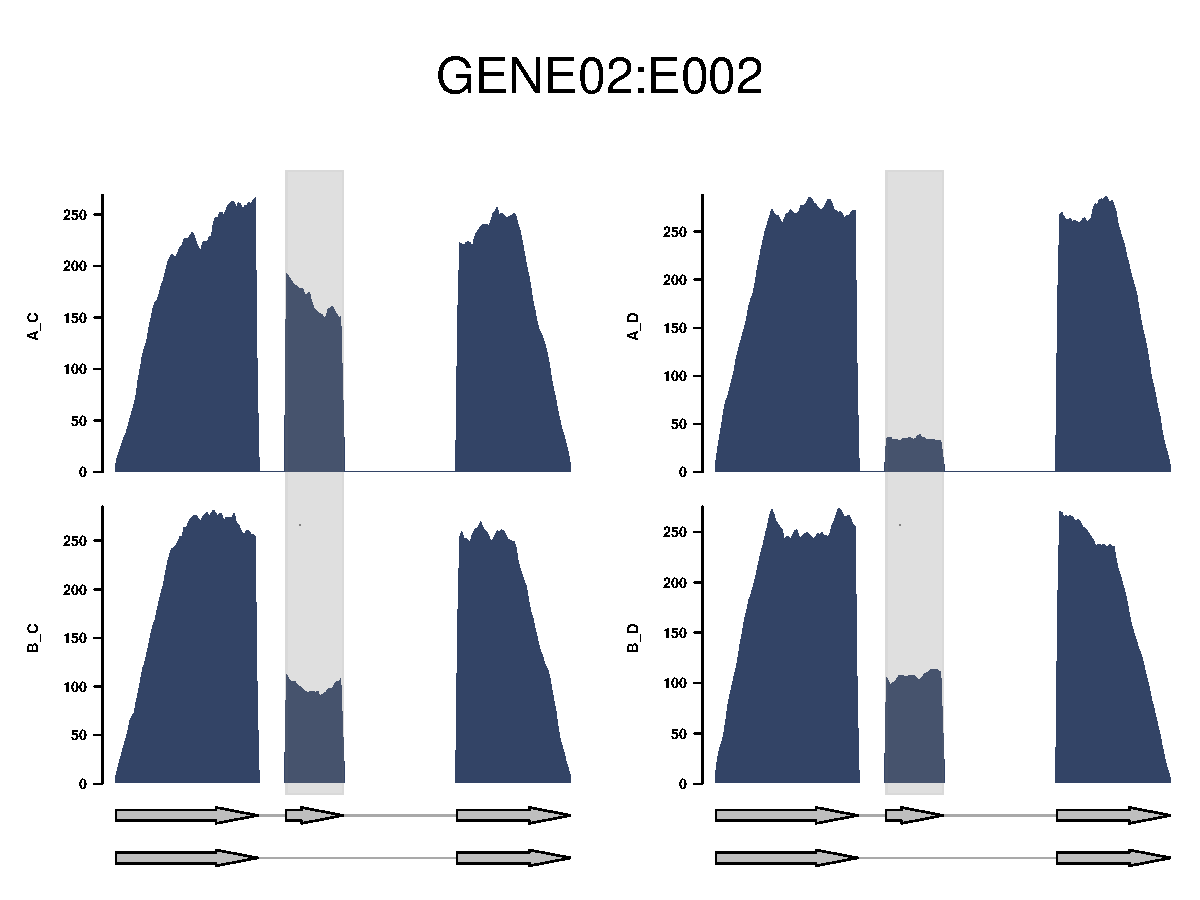
\includegraphics[width=0.6\textwidth]{images/GENE02_E002_gr.pdf}
  \end{center}
  \caption{Genomic plot of a gene containing a exon skipping splicing event
  highlighted for four different conditions.}
  \label{fig:plotGenomicRegion}
\end{figure}

In addition to coverage plots, \texttt{ASpli} is able to draw plots containing
raw gene counts, raw bin counts, PSI/PIR value, inclusion and exclusion junction
counts for a single bin in all, or a subset, conditions of the analysis. This
plot is useful to integrate evidences of different sources in order to explain
an experimental result. The function to make these plots is \texttt{plotBins},
below there are some examples of use.

Example 1:
<<plotbins, echo=TRUE, eval=FALSE>>=
# Defines an experiment with one experimental factor (genotype, with two
# values: wild-type (WT) and mutant (MT) ), and three replicate samples for each
# condition.
targets <- data.frame(
  row.names = c( 'WT1', 'WT2', 'WT3', 
                 'MT1', 'MT2', 'MT3' ),
  bam = c( 'WT1.bam', 'WT2.bam', 'WT3.bam', 
           'MT1.bam', 'MT2.bam', 'MT3.bam' ),
  genotype = c( 'WT','WT','WT','MT','MT','MT' ),
  stringsAsFactors = FALSE )
# Specifies what factors and values will be plotted, in this example all of
# them.
fv = list( genotype = c( 'WT', 'MT' ) ) 
plotbins(
        counts, 
        as,
        'GENE02:E002', 
        factorsAndValues = fv, 
        targets )
@

Example 2:
<<plotbins, echo=TRUE, eval=FALSE>>=
# Defines an experiment with two experimental factor (treat, with four
# values: A, B, C and D; and time, with twelve values from T1 to T12.), and
# two replicate samples for each condition. In the definition, many values are
# not shown to reduce the space of the example, and are replaced by '...' . 
targets <- data.frame(
  row.names = c( 'A_T1.r1', 'A_T1.r2', 
                 'A_T2.r1', 'A_T2.r2',
                 ... , 
                 'D_T12.r1', 'D_T12.r2' ),
  bam = c( 'A_T1.r1.bam', 'A_T1.r2.bam', 
           'A_T2.r1.bam', 'A_T2.r2.bam',
           ... , 
           'D_T12.r1.bam', 'D_T12.r2.bam' ),
  treat = c( 'A', 'A',
             'A', 'A',
             ... ,
             'D', 'D' ),
  time = c( 'T1', 'T1',
            'T2', 'T2,
            ... ,
            'T12', 'T12' ),
  stringsAsFactors = FALSE )
# Draw the plots.
plotbins(
        counts, 
        as,
        'GENE02:E002', 
        factorsAndValues = fv, 
        targets )

# Specifies what factors and values will be plotted. In this example there are
# two factor, the first one in 'fv' list is the main factor, values will
# be grouped by this factor. 
fv = list( time = c( 'T1', 'T2', ... , 'T12' ) ,
           treat = c( 'A', 'B', 'C', 'D' ) ) 
# Draw the plots
plotbins(
        counts, 
        as,
        'GENE02:E002', 
        factorsAndValues = fv, 
        targets )
@

Figures \ref{fig:plotbinEx1} and \ref{fig:plotbinEx2} shows the images that can
be obtained in setups like shown in the examples above. Note that one image contains barplots, and the
other contains lines, they are selected automatically according to the number of
conditions and values per condition. However, it is possible to force to one of
them.

\begin{figure}
  \includegraphics[width=0.6\textwidth]{ }
  \caption{}
  \label{fig:plotbinEx1} 
\end{figure}

\begin{figure}
  \includegraphics[width=0.6\textwidth]{ }
  \caption{}
  \label{fig:plotbinEx2} 
\end{figure}

\subsection{Utility functions}

\section{Example data}
It is possible to run a demo of \texttt{ASpli} using public RNA-seq data available via Bioconductor. It requieres installing of \texttt{RNAseqData.HNRNPC.bam.chr14} package and loading  an small TranscriptDb of Human Genome only for chromosome 14. This subset of reads is part of an experiment intended to analyze splicing factors and their relationship with exonization of Alu elements \cite{Zarnack2013453}. We load the package and the genome:
%<<librariesEx, echo=TRUE, eval=TRUE>>=
<<librariesEx, echo=TRUE, eval=FALSE>>=
library(RNAseqData.HNRNPC.bam.chr14)
@

In this case we are loading a genome \texttt{TranscriptDb} already created and available in the  \texttt{ASpli} package for the Homo sapiens chromosome 14:

%<<loadDb, echo=TRUE, eval=TRUE>>=
<<loadDb, echo=TRUE, eval=FALSE>>=
chr14 <- system.file("extdata","chr14.sqlite", package="ASpli")
genome <- loadDb(chr14)
@

And now we are ready to start the complete analysis.
%<<binGenome, echo=TRUE, eval=TRUE>>=
<<binGenome, echo=TRUE, eval=FALSE>>=
features <- binGenome(genome) 
@

Create targets object using the information of the available files:
%<<targetsEx, echo=TRUE, eval=TRUE>>=
<<targetsEx, echo=TRUE, eval=FALSE>>=
targets <- data.frame(bam=RNAseqData.HNRNPC.bam.chr14_BAMFILES,
                       condition=c(rep("CT",4),rep("KD",4)))
@
Load bam files:
%<<loadBam, echo=TRUE, eval=TRUE>>=
<<loadBam, echo=TRUE, eval=FALSE>>=
bam <- loadBAM(targets)
@
Overlap alignments against features:
%<<todosJuntos, eval=TRUE>>=
<<todosJuntos, eval=FALSE>>=
counts<-readCounts(features, bam, targets, readLength=100L, maxISize=50000)
@
Perform DE/DU analysis
%<<DU, eval=TRUE>>=
<<DU, eval=FALSE>>=
du_HNRNPC <- DUreport(counts, targets)
@
Analyze AS using junctions:
%<<AS, eval=TRUE>>=
<<AS, eval=FALSE>>=
as_HNRNPC <- AsDiscover (counts, targets, features, bam, readLength=100L, threshold = 5, cores = 1 )
@

Select TopTags (only using DU information:)
%<<topTags, echo=TRUE, eval=TRUE>>=
<<topTags, echo=TRUE, eval=FALSE>>=
binsdu <- binsDU(du_HNRNPC)
topTagsBins <- which(binsdu$bin.fdr <= 0.1 & 
                 abs(binsdu$logFC) >=0.58)
@

We can inspect visually the results of topTags. Sometimes is useful to merge BAM files by conditions. \textit{(In this example data, control and knock down replicates were  merged using \texttt{samtools merge} into \textbf{CT.bam} and \textbf{KD.bam} respectively)}.

%<<targetsPlot, eval=TRUE>>=
<<targetsPlot, eval=FALSE>>=
targetsPlot <- data.frame(bam=targets$bam, 
                        sample=targets$condition, 
                        color=c(rep("blue", 4),rep("red", 4)), 
                        stringsAsFactors=FALSE)
@

%<<auxdf, echo=TRUE, eval=TRUE>>=
<<auxdf, echo=TRUE, eval=FALSE>>=
auxdf<-binsdu[topTagsBins,]
#for simplicity, we choose one: LRR1:E005
plotTopTags(auxdf["LRR1:E005",], 
            genome, 
            targetsPlot, 
            output.dir="testPlots")
@
\begin{figure}[ht!]
\centering
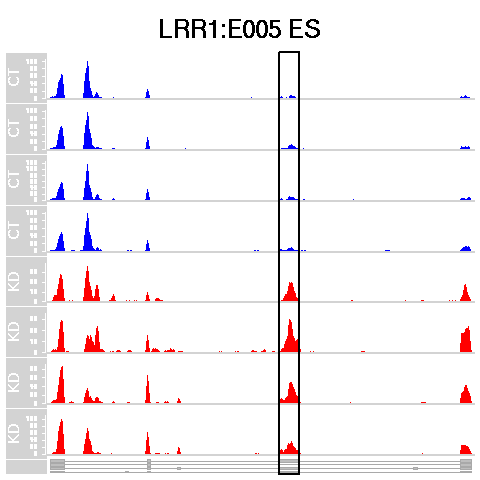
\includegraphics[width=0.5\textwidth]{LRR1_E005.png}
\caption{Plot of LRR1:E005 Exon Skipping}
\end{figure}


%<<check, echo=TRUE, eval=TRUE>>=
<<check, echo=TRUE, eval=FALSE>>=
binsdu <- binsDU(du_HNRNPC)
topTagsBins <- which(binsdu$bin.fdr <= 0.1 & 
                     abs(binsdu$logFC) >=0.58)
@

%<<sessionInfo, eval=TRUE, echo=TRUE>>=
<<sessionInfo, eval=FALSE, echo=TRUE>>=
sessionInfo()
@

\bibliography{ASpli}
\end{document}
